% FACULTAD DE INGENIERÍA, UNIVERSIDAD DE BUENOS AIRES

\documentclass[a4paper]{article}
\usepackage[spanish]{babel}
\usepackage[utf8x]{inputenc}
\usepackage{amsmath}
\usepackage{amssymb}
\usepackage{graphicx}
\usepackage{float}
\usepackage{dcolumn}
\title{Trabajo Especial}
\author{Alumnos}

%para los boxes de los enunciados.
\usepackage{framed}
%para hacer que los items del índice y las referencias a imagenes sean links
\usepackage{hyperref}
\hypersetup{
    colorlinks,
    citecolor=black,
    filecolor=black,
    linkcolor=black,
    urlcolor=black,
}


%para insertar enunciados
\newenvironment{enunciado}{
\begin{leftbar}
\textbf{Enunciado:}
\itshape}{
\end{leftbar}
}


\begin{document}

\setlength{\unitlength}{1 cm} %Especificar unidad de trabajo
\thispagestyle{empty}
\begin{picture}(5,4)
\put(-1,0){
\includegraphics{./imagenes/fiuba}}
\end{picture}

\vspace{1cm}

\begin{center}
\textbf{{\LARGE Circuitos Electrónicos I [66.08]}\\[0.5cm]
{\Large Julio G. Zola}}\\[1.25cm]

{\Large \textbf{Informe: Trabajo de Laboratorio IV \\[1.25cm]
Diseño Analógico: Robot seguidor de líneas.
}}

\vspace{1cm}
{\textbf{Primer Cuatrimestre 2014\\[1.25cm]
}}
\vspace{1cm}

\begin{tabbing}
\hspace*{3cm} \= \hspace*{3cm} \= \hspace*{3cm}\= \hspace*{3cm} \kill
\textbf{Nombre} \> \textbf{Apellido} \> \textbf{Padrón} \> \textbf{Mail} \\
 \>  \>  \>  \\
Iván Gustavo\> Pollitzer \> 82957\> igpollitzer@gmail.com\\
Ignacio L. J. \> Carballeda \> 91646\> carballeda.ignacio@gmail.com\\
\end{tabbing}
%I. L. J. Carballeda, parece un escritor de novelas de fantasía heroica

\end{center}


\newpage

\tableofcontents

\newpage


\section{ \textbf{Introducción}}


El objetivo de este trabajo es realizar un robot seguidor de líneas utilizando componentes analógicos.
Un seguidor de líneas es un simple robot móvil, ideal para los que se inician en la robótica. Tal es así que es considerado el ''hola mundo'' del mundo robotico.\\

Básicamente el objetivo del robot es seguir una línea que describe un circuito cerrado.
Para la implementación de este tipo de robot generalmente se utilizan microcontroladores ya que permiten tomar decisiones mas ''inteligentes'' para recorrer la pista en el menor tiempo posible.


\begin{figure}[H]
  \centering
    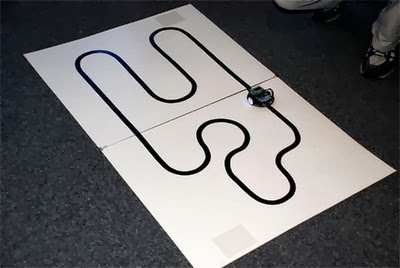
\includegraphics[width=\textwidth]{./imagenes/robot_ejemplo.jpg}
  \caption{Robot seguidor de lineas.}
\end{figure}

\newpage

\subsection{Idea de funcionamiento}

El circuito sobre el cual se tiene que desplazar el robot consta de una linea blanca (brillante) con fondo negro (opaco).\\

El robot es dotado de dos sensores ubicados de manera tal que puedan medir el suelo y dos motores que funcionan de manera independiente. 
La idea es que cuando ambos sensores estén sobre la línea, el robot avance de manera recta. Cuando, por ejemplo, el sensor del lado derecho salga de la línea,
el motor izquierdo detiene su marcha, haciendo de esta manera que el vehículo gire hacia la izquierda para volver sobre la línea blanca.


\begin{figure}[H]
  \centering
    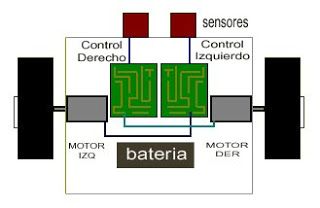
\includegraphics[width=\textwidth]{./imagenes/autito.jpg}
  \caption{idea}
\end{figure}

\newpage

\section{Sensores}

Para permitir que el robot pueda distinguir la línea blanca del fondo negro utilizamos dos sensores CNY70.\\
El CNY70 es un sensor de corto alcance, compuesto por un emisor de luz (diodo infrarrojo) y un receptor (foto-transistor), ambos apuntando en la misma dirección. Su funcionamiento se basa en la capacidad de reflexión del objeto,
y la detección del rayo reflectado por el receptor.\\

El mismo tiene cuatro pines de conexión. Dos de ellos se corresponden con el ánado y cátodo del emisor, y las otras dos se corresponde con el colector y el emisor del receptor.

\begin{figure}[H]
  \centering
    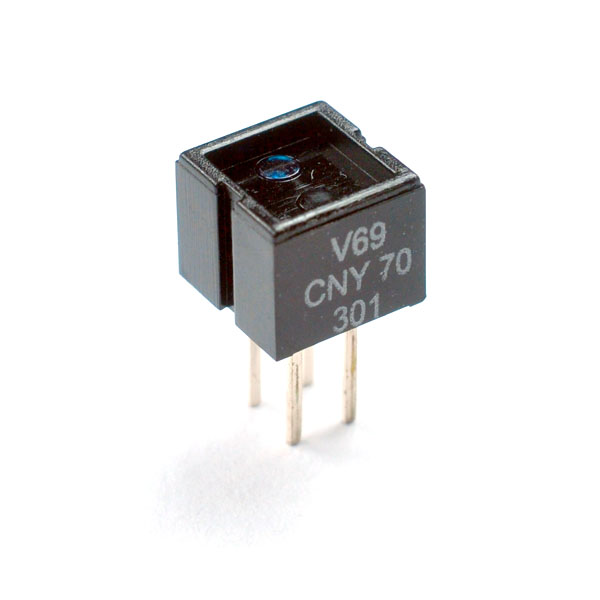
\includegraphics[width=\textwidth]{./imagenes/cny70.jpg}
  \caption{CNY70}
\end{figure}


\section{Circuito utilizado}


\subsection{Requerimientos}

Los motores sometidos a una diferencia de potencial de 4 $V$ consumen 40 $mA$, cuando están funcionando libremente. 
En cambio, cuando están siendo bloqueados físicamente, consumen 250 $mA$.

Necesitamos un circuito que entregue una corriente de 250 $mA$ (peor caso) cuando el sensor detecte la línea blanca.

\subsection{Explicación de la elección del circuito}

Cuando la luz infrarroja emitida por el foto-diodo es reflejada por la superficie blanca de la línea, la base del foto-transistor (TBJ NPN) es excitada.
Cuando esto sucede, la corriente por el mismo se eleva y produce un incremento de tensión en el emisor, ya que el mismo esta conectado a un resistor de 10 $K\omega$
que va a tierra.\\

La idea es medir la tensión en el emisor del foto-diodo y transformarla, de alguna manera, en corriente circulando por el motor correspondiente.\\

\begin{figure}[H]
  \centering
    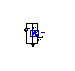
\includegraphics[width=\textwidth]{./xcircuit/definiendo1.eps}
  \caption{circuito}
\end{figure}

Como no queremos tomar corriente del foto-diodo ya que esto provocaria su ruptura (corriente máxima $I_{c_{sensor}}=50$ $mA$). Lo primero que se nos ocurrió
fue conectar la base de un transistor TBJ al nodo emisor del sensor como se muestra en la siguiente figura.

\begin{figure}[H]
  \centering
    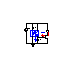
\includegraphics[width=\textwidth]{./xcircuit/definiendo2.eps}
  \caption{circuito propuesto}
\end{figure}

Cuando el sensor detecta la línea blanca $I_{c_{sensor}}=\frac{4 V}{10 K \Omega}= 0.4$ $mA$ .\\
Cuando el motor esta bloqueado $I_c=250$ $mA$, por lo tanto con un $\beta_{min}=85$ , $I_{b}=\frac{250 mA}{85}\simeq 3 mA$. \\
Como vemos el problema esta en que no podemos sacar esos 3 $mA$ directamente del sensor. Si comparamos esta corriente 
con la que esta circulando por el foto-transistor veremos que no es despreciable y esto afectaría nuestra medición.\\

Para solucionar este problema decidimos conectar el gate de un transistor N-MOSFET con una tensión de umbral
lo suficientemente baja ($v_{th}= 1$ $V$) al emisor del foto-transistor.\\
Esta decisión en principio solucionaría el problema de sacar corriente del foto-transistor. Esto es porque la corriente por gate en un MOS es casi nula.\\

Sin embargo ahora nos enfrentamos con otro problema. La corriente necesaria para hacer funcionar un motor excede los valores típicos de $I_D$ de los mosfet.\\
Por esta razón se conecto el drain del NMOS a la base de un TBJ de tipo PNP. De esta forma podríamos utilizar corrientes bajas,
para controlar corrientes mas altas por TBJ. \\
El circuito quedo de la siguiente manera:

\begin{figure}[H]
  \centering
    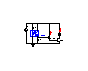
\includegraphics[width=\textwidth]{./xcircuit/Page_1.eps}
  \caption{circuito propuesto}
\end{figure}

Cuando realizamos las mediciones nos dimos cuenta que la corriente $ID$ del MOS era mucho mas alta de la que esperábamos $I_D\approx 200$ $mA$.
Observamos que el motor funcionaba correctamente pero que el MOS se calentaba demasiado.\\

El circuito estaba funcionando ya que el TBJ estaba saturado y permitía la corriente necesaria por el motor. Pero era innecesariamente excesiva, la corriente
que estaba circulando por el Drain del MOS. \\

Con una corriente por Drain de 3 $mA$ ya es suficiente dado que\\
$I_C=\beta_{min}*I_D=85*3$ $mA$ = 255 $mA$.\\
La resistencia que impone el canal formado a la corriente continua es de aproximadamente 100 $\Omega$. Despejando: \\

\begin{equation*}
 I_D=\frac{4 - 0.7}{ 100 \Omega + R_D } = 3 mA \Longrightarrow R_D= 1 K \Omega 
\end{equation*}

Por lo tanto agregamos un resistor $R_D=1$ $K \Omega$ 
entre el Drain del MOS y VCC.\\

Los transistores que elegimos fueron sobredimensionados para cubrirnos ante posibles fallas.\\
\begin{itemize}
  \item  TBJ = NPN BD329 (Corriente máx = 3 $A$,  disipación máx =  15 $W $ , $ 85 \leqq h_{fe} \leqq 375 $ )
  \item  MOS = NMOS BSS88 ($I_{D_{max}}=250$ $mA$ , disipación = 1 W, $0.6 V \leqq v_{th}\leqq 1.6 V$ ,$10 nA \leqq I_{GSS}\leqq 100 nA $ )
\end{itemize}

Quedando finalmente el circuito configurado de la siguiente manera:

\begin{figure}[H]
  \centering
    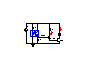
\includegraphics[width=\textwidth]{./xcircuit/Page_2.eps}
  \caption{circuito final}
\end{figure}

\section{Mediciones}

\subsection{Mediciones sobre TBJ}

\begin{tabular}{||l | c | r | r ||}
\hline
\hline
Color & Motor & $V_{CE}$ & $I_C$ \\
\hline
Blanco & libre & 18 $mV$ & 41 $mA$ \\
\hline
Blanco & bloqueado & 81 $mV$ & 195 $mA$\\
\hline
Negro & libre & 4.13 $V$ & 0 $A$\\
\hline
\end{tabular}

\subsection{Mediciones sobre MOSFET}

\begin{tabular}{||l | c | r | r | r||}
\hline
\hline
Color & Motor & $V_{DS}$ & $I_D$ & $V_G$\\
\hline
Blanco & libre & 13 $mV$ & 3.4 $mA$ & 3.92 $V$ \\
\hline
Blanco & bloqueado & 12.8 $mV$ & 3.3 $mA$ & 3.92 $V$ \\
\hline
Negro & libre & 3.64 $V$ & 0 $A$ & 34 $mV$ \\
\hline
\end{tabular}


\end{document}